% \begin{table*}[t]
\centering
\resizebox{\linewidth}{!}{%
\begin{tabular}{l|c|cccc|ccc|c|c}
\toprule[1pt]
\multirow{2}{*}{\textbf{Method}} & \multirow{2}{*}{\textbf{Overall $\uparrow$}} & \multicolumn{4}{c|}{\textbf{Performance by Type $\uparrow$}} & \multicolumn{3}{c|}{\textbf{Build Tokens (M) $\downarrow$}} & \multirow{2}{*}{\textbf{Calls $\downarrow$}} & \multirow{2}{*}{\textbf{Time (s) $\downarrow$}} \\
\cmidrule(lr){3-6} \cmidrule(lr){7-9}
& & \textbf{Multi} & \textbf{Open} & \textbf{Single} & \textbf{Temp} & \textbf{In} & \textbf{Out} & \textbf{Sum} & & \\
\midrule
%--- RAG Methods (Gray Background) ---
\rowcolor{RAGColor} OpenAI & 71.82 & 69.86 & 53.12 & \underline{84.66} & 45.48 & -- & -- & -- & -- & -- \\
\rowcolor{RAGColor} FullContext &73.83	&68.79	&56.25	&\textbf{86.56}	&50.16 & -- & -- & -- & -- & -- \\
% \rowcolor{RAGColor} NaiveRAG & 63.64 &55.32	&47.92	&70.99	&56.39 & -- & -- & -- & -- & -- \\
\rowcolor{RAGColor} MiniRAG & 63.51 & 56.74 & 58.33 & 75.74 & 38.94 & 9.022 & 1.081 & 10.103 & \underline{2508} & \textbf{2566} \\
\rowcolor{RAGColor} LightRAG & 68.83 & 66.31 & 50.00 & 77.53 & 53.89 & 10.014 & 1.916 & 11.931 & 13576 & 60469 \\
\midrule
% --- Memory Methods (Blue Background) ---
% \rowcolor{MemoryColor} LightMem & 74.74 & 66.67 & 45.83 & 79.31 & 78.50 & \textbf{0.770} & \textbf{0.178} & \textbf{0.948} & \textbf{387} & \textbf{14560} \\
\rowcolor{MemoryColor} LangMem & 58.10 & 62.23 & 47.92 & 71.12 & 23.43 & 9.873 & 1.192 & 11.066 & 5990 & 26281 \\
\rowcolor{MemoryColor} A-Mem &64.16	&56.03	&31.25	&72.06	&60.44 & 9.126 & 2.368 & 11.494 & 11754 & 60607 \\
\rowcolor{MemoryColor} Mem0 &66.88 &67.13 & 51.15	&72.93 &59.19 & 10.958 & 1.239 & 12.196 & 9181 & 30057 \\
% --- Structural Memory Methods (Purpl Background) ---

\midrule
\rowcolor{StructuralMemoryColor} MemoryOS & 58.25 & 56.74	& 45.83	& 67.06	& 40.19 & \underline{1.889} & \underline{0.939} & \underline{2.868} & 5534 & 24220\\
\rowcolor{StructuralMemoryColor} 
$\text{Mem0}^\text{g}$ & 68.44 &65.71 &47.19 &75.71	&58.13 & 33.512 & 2.313 & 35.825 & 53514 & 115670 \\
\rowcolor{StructuralMemoryColor} Zep & 75.14 & \textbf{74.11} & \textbf{66.04} & 79.79 & 67.71 & -- & -- & -- & -- & -- \\
\rowcolor{StructuralMemoryColor} Memobase & \underline{75.78} & \underline{70.92} & 46.88 & 77.17 & \textbf{85.05} & -- & -- & -- & -- & -- \\
\rowcolor{StructuralMemoryColor} \textbf{StructMem} & \textbf{76.82} & 68.77 & 46.88 & 81.09 & \underline{81.62} & \textbf{1.501} & \textbf{0.436} & \textbf{1.937} & \textbf{1056} & \underline{22854} \\
\bottomrule[1pt]
\end{tabular}
} 
\caption{Performance and resource consumption comparison of memory systems on \texttt{LoCoMo} dataset. $\uparrow$: larger is better; $\downarrow$:  smaller is better.  \textbf{The best results} are marked in bold,  \underline{the second-best results} are underlined. Row colors distinguish method categories: \colorbox{RAGColor}{RAG methods}, \colorbox{MemoryColor}{Flat Memory methods}, and \colorbox{StructuralMemoryColor}{Structural Memory methods}. OpenAI and FullContext have no construction cost; Zep and Memobase do not expose construction details.}
\label{tab:locomo}
\end{table*}

\section{Method}
% \yunzhi{You need to add Memory Extraction/Memory Refinement in the Figure 2.}


\begin{figure*}[!t]
    \centering
    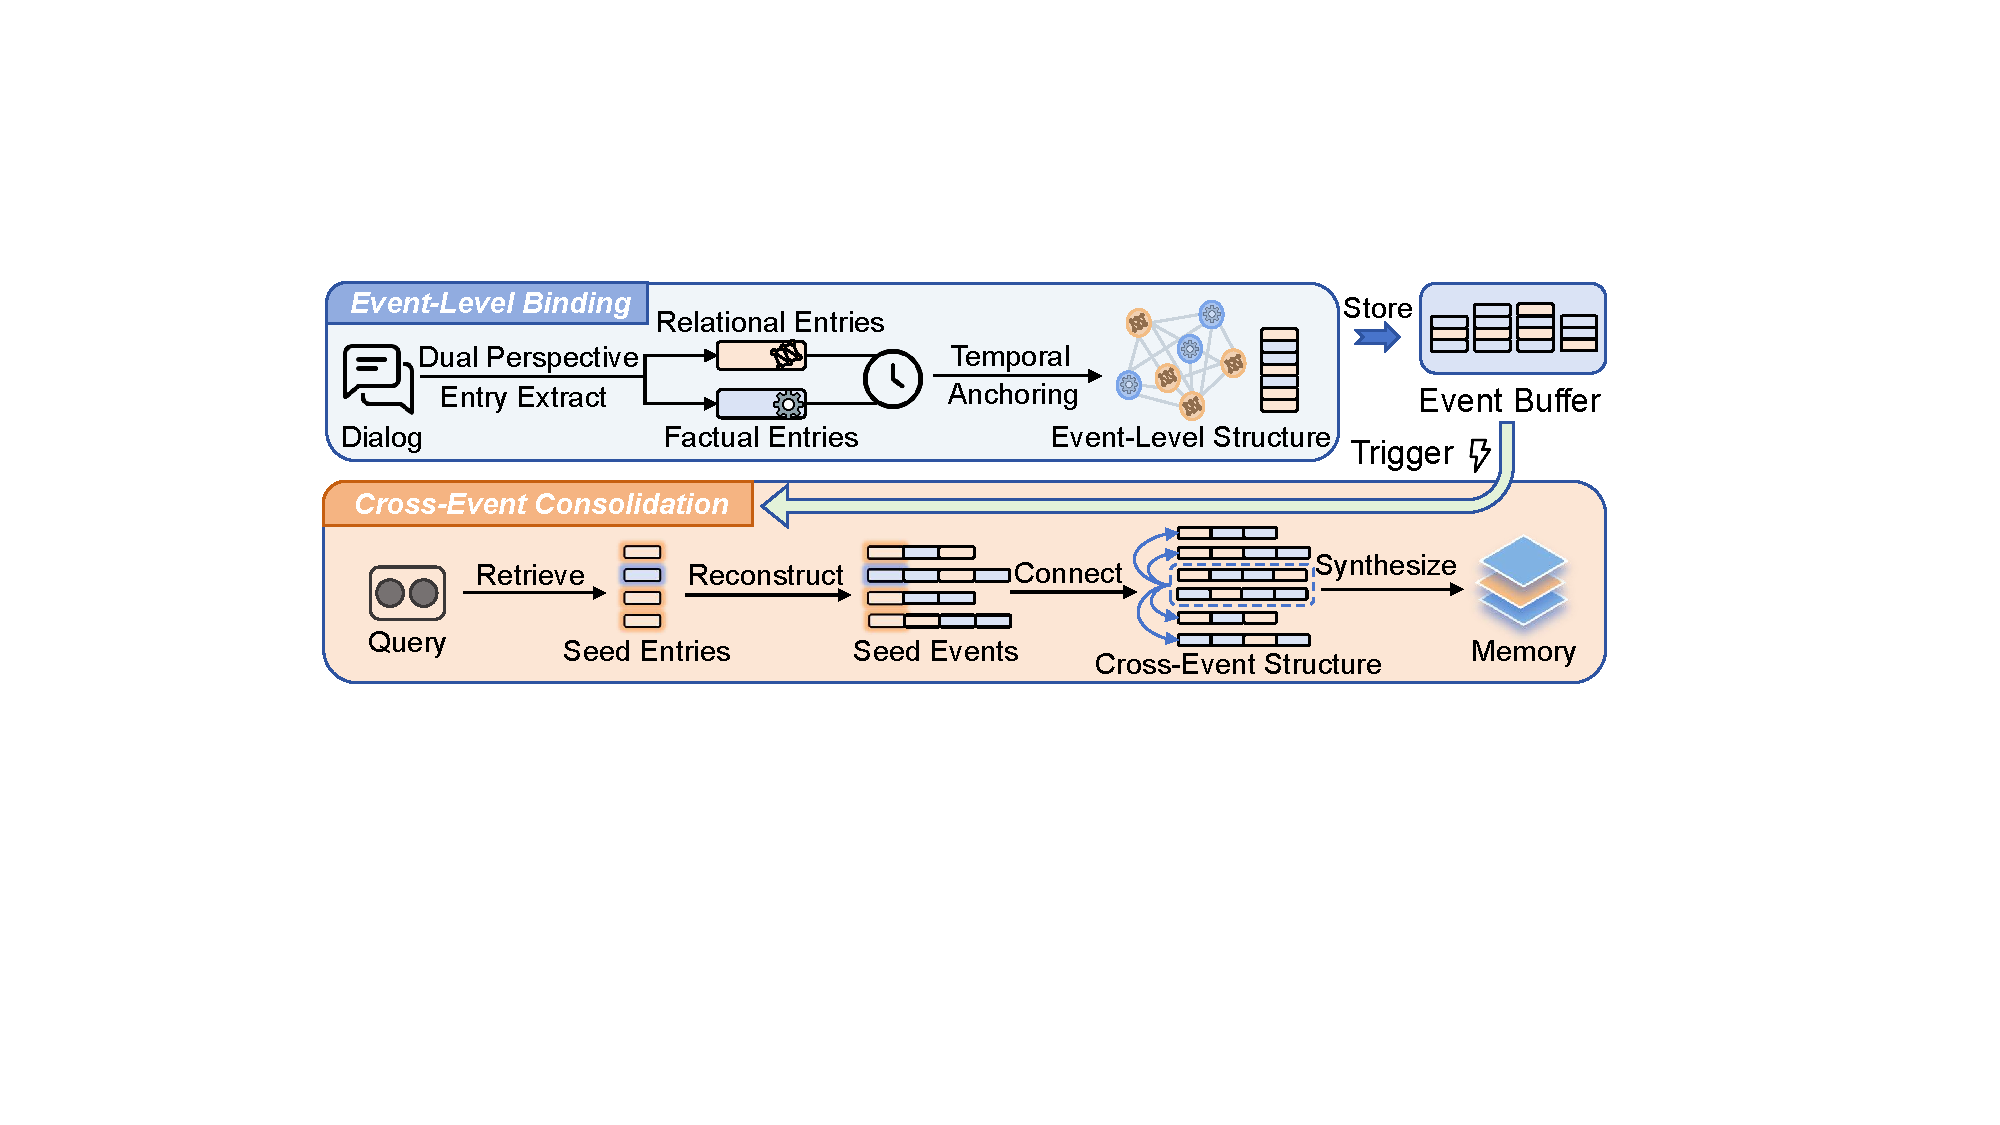
\includegraphics[width=1.0\linewidth]{figure/2026ACL-Demo.pdf}
    \caption{StructMem's hierarchical memory organization. \textbf{Event-Level Binding} constructs event-level structure by extracting dual perspectives and anchoring them temporally. \textbf{Cross-Event Consolidation} constructs cross-event structure through semantic retrieval, event reconstruction, and consolidation synthesis.}
    \label{fig:overview}
\end{figure*}


We propose \textbf{StructMem}, a framework that achieves structure-enriched organization through hierarchical design. The framework operates at two levels: event-level structure (\S\ref{sec:event-level}) preserves relational bindings within individual utterances, while cross-event structure (\S\ref{sec:cross-event}) connects information across temporal boundaries.

\subsection{Event-Level Binding}
\label{sec:event-level}
Event-level binding preserves the connection between factual content and relational context within individual utterances through dual-perspective extraction and temporal anchoring.

\textbf{Dual-Perspective Extraction.} 
For each utterance $m_i$ in the dialogue stream, we extract entries from two complementary perspectives using language model $\mathcal{L}$ with prompts $P_{fact}$ and $P_{rel}$:
\begin{equation}
\Phi_i \cup \Psi_i = \mathcal{L}( P_{fact} \| m_i ) \cup \mathcal{L}( P_{rel} \| m_i ),
\end{equation}
where $\Phi_i = \{c_{i,1}, \ldots, c_{i,j}\}$ contains \textit{factual entries} describing event content, and $\Psi_i = \{r_{i,1}, \ldots, r_{i,k}\}$ contains \textit{relational entries} capturing interpersonal dynamics, causal influences, and temporal dependencies. 
 
By representing both in natural language rather than rigid triplets, we preserve the contextual nuances required for episodic grounding while avoiding entity resolution overhead.
  
\textbf{Temporal Anchoring.}
To preserve the binding between relational and factual information, all entries are anchored to their originating timestamp $\tau_i$, forming an event-level unit:
\begin{equation}
\mathcal{M} \leftarrow  \bigcup_{i=1}^{N} \left\{ \langle x, \mathbf{e}_x, \tau_i \rangle \mid x \in \Phi_i \cup \Psi_i \right\},
\end{equation}
where $\mathbf{e}_x$ denotes the embedding of entry $x$. This temporal coupling enables reconstruction of complete factual-relational events during retrieval.

\begin{table*}[t]
\centering
\resizebox{\linewidth}{!}{%
\begin{tabular}{l|c|cccc|ccc|c|c}
\toprule[1pt]
\multirow{2}{*}{\textbf{Method}} & \multirow{2}{*}{\textbf{Overall $\uparrow$}} & \multicolumn{4}{c|}{\textbf{Performance by Type $\uparrow$}} & \multicolumn{3}{c|}{\textbf{Build Tokens (M) $\downarrow$}} & \multirow{2}{*}{\textbf{Calls $\downarrow$}} & \multirow{2}{*}{\textbf{Time (s) $\downarrow$}} \\
\cmidrule(lr){3-6} \cmidrule(lr){7-9}
& & \textbf{Multi} & \textbf{Open} & \textbf{Single} & \textbf{Temp} & \textbf{In} & \textbf{Out} & \textbf{Sum} & & \\
\midrule
%--- RAG Methods (Gray Background) ---
\rowcolor{RAGColor} OpenAI & 71.82 & 69.86 & 53.12 & \underline{84.66} & 45.48 & -- & -- & -- & -- & -- \\
\rowcolor{RAGColor} FullContext &73.83	&68.79	&56.25	&\textbf{86.56}	&50.16 & -- & -- & -- & -- & -- \\
% \rowcolor{RAGColor} NaiveRAG & 63.64 &55.32	&47.92	&70.99	&56.39 & -- & -- & -- & -- & -- \\
\rowcolor{RAGColor} MiniRAG & 63.51 & 56.74 & 58.33 & 75.74 & 38.94 & 9.022 & 1.081 & 10.103 & \underline{2508} & \textbf{2566} \\
\rowcolor{RAGColor} LightRAG & 68.83 & 66.31 & 50.00 & 77.53 & 53.89 & 10.014 & 1.916 & 11.931 & 13576 & 60469 \\
\midrule
% --- Memory Methods (Blue Background) ---
% \rowcolor{MemoryColor} LightMem & 74.74 & 66.67 & 45.83 & 79.31 & 78.50 & \textbf{0.770} & \textbf{0.178} & \textbf{0.948} & \textbf{387} & \textbf{14560} \\
\rowcolor{MemoryColor} LangMem & 58.10 & 62.23 & 47.92 & 71.12 & 23.43 & 9.873 & 1.192 & 11.066 & 5990 & 26281 \\
\rowcolor{MemoryColor} A-Mem &64.16	&56.03	&31.25	&72.06	&60.44 & 9.126 & 2.368 & 11.494 & 11754 & 60607 \\
\rowcolor{MemoryColor} Mem0 &66.88 &67.13 & 51.15	&72.93 &59.19 & 10.958 & 1.239 & 12.196 & 9181 & 30057 \\
% --- Structural Memory Methods (Purpl Background) ---

\midrule
\rowcolor{StructuralMemoryColor} MemoryOS & 58.25 & 56.74	& 45.83	& 67.06	& 40.19 & \underline{1.889} & \underline{0.939} & \underline{2.868} & 5534 & 24220\\
\rowcolor{StructuralMemoryColor} 
$\text{Mem0}^\text{g}$ & 68.44 &65.71 &47.19 &75.71	&58.13 & 33.512 & 2.313 & 35.825 & 53514 & 115670 \\
\rowcolor{StructuralMemoryColor} Zep & 75.14 & \textbf{74.11} & \textbf{66.04} & 79.79 & 67.71 & -- & -- & -- & -- & -- \\
\rowcolor{StructuralMemoryColor} Memobase & \underline{75.78} & \underline{70.92} & 46.88 & 77.17 & \textbf{85.05} & -- & -- & -- & -- & -- \\
\rowcolor{StructuralMemoryColor} \textbf{StructMem} & \textbf{76.82} & 68.77 & 46.88 & 81.09 & \underline{81.62} & \textbf{1.501} & \textbf{0.436} & \textbf{1.937} & \textbf{1056} & \underline{22854} \\
\bottomrule[1pt]
\end{tabular}
} 
\caption{Performance and resource consumption comparison of memory systems on \texttt{LoCoMo} dataset. $\uparrow$: larger is better; $\downarrow$:  smaller is better.  \textbf{The best results} are marked in bold,  \underline{the second-best results} are underlined. Row colors distinguish method categories: \colorbox{RAGColor}{RAG methods}, \colorbox{MemoryColor}{Flat Memory methods}, and \colorbox{StructuralMemoryColor}{Structural Memory methods}. OpenAI and FullContext have no construction cost; Zep and Memobase do not expose construction details.}
\label{tab:locomo}
\end{table*}

\subsection{Cross-Event Consolidation}
\label{sec:cross-event} 
Cross-event consolidation connects information across temporal by periodically synthesizing semantically related events. We trigger synthesis when accumulated events exceed a time threshold.

\textbf{Semantic Event Connections.} 
We buffer unconsolidated entries since the last consolidation. The buffered entries are temporally ordered:
\begin{equation}
\mathcal{C}_{buf} = \text{Sort}_{\tau} \{ x \in \mathcal{M}_{buffer} \},
\end{equation}
where $\mathcal{M}_{buffer}$ denotes the buffered entries. We encode the buffered context into an aggregated query by concatenating all buffered entry texts and encoding them with an embedding model. We then rank all historical entries by cosine similarity to this query and retrieve the top-$K$ most semantically similar entries as seeds, denoted as $\mathcal{S}_k$.

For each seed entry $x^* \in \mathcal{S}_k$, we reconstruct its complete event context by retrieving all entries sharing the same timestamp:
\begin{equation}
{E}_{\tau}(x^*) = \{ x' \in \mathcal{M} \mid \tau(x') = \tau(x^*) \}.
\end{equation}
These reconstructed events, together with the buffered events, form the cross-event structure grounded in semantic relevance.
\begin{equation}
\mathcal{C}_{cross} = \mathcal{C}_{buf} \cup \bigcup_{x^* \in \mathcal{S}_k} {E}_{\tau}(x^*).
\end{equation}
\textbf{Memory Consolidation through Synthesis.} 
Unlike conventional summarization that performs lossy compression on sequential text, our consolidation mechanism operates on semantically-reconstructed event clusters. It explicitly synthesizes cross-event relational hypotheses, forming a complementary abstraction layer that enables multi-hop reasoning while faithfully preserving the fidelity of raw episodic memory.
\begin{equation}
\mathcal{M} \leftarrow \mathcal{C}_{cons} = \mathcal{L}( P_{cons} \| \mathcal{C}_{cross} ).
\end{equation}